\documentclass{article}
\usepackage{amsmath}
\usepackage{tikz}
\usetikzlibrary{arrows.meta}

\begin{document}

\begin{equation*}
\tau \; : \quad 
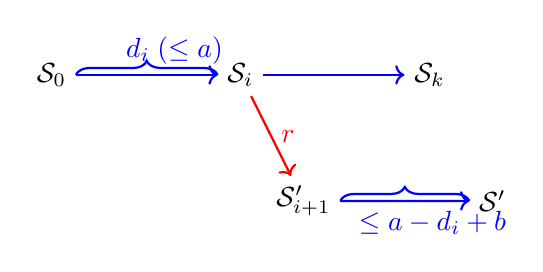
\begin{tikzpicture}[baseline=(current bounding box.center), scale=0.8]
    \node (s0) at (0,0) {$\mathcal{S}_0$};
    \node (si) at (3,0) {$\mathcal{S}_i$};
    \node (sk) at (6,0) {$\mathcal{S}_k$};
    \node (sip1) at (4,-2) {$\mathcal{S}_{i+1}'$};
    \node (sprime) at (7,-2) {$\mathcal{S}'$};

    \draw[->, thick, blue] (s0) -- node [above] {} (si);
    \draw[->, thick, blue] (si) -- node [above] {} (sk);
    \draw[->, thick, blue] (sip1) -- node [above] {} (sprime);

    \draw[->, thick, red] (si) -- node [right] {$r$} (sip1);

    \draw[decorate, decoration={brace, amplitude=5pt}, thick, blue] (s0) -- node [midway, above, xshift=1em] {$d_i \; (\leq a)$} (si);
    \draw[decorate, decoration={brace, amplitude=5pt}, thick, blue] (sip1) -- node [midway, below, xshift=1em] {$\leq a - d_i + b$} (sprime);
\end{tikzpicture}
\end{equation*}

An $(n,a,b)$-resilient trace $\tau$ and an $(n-1,a-d_i,b)$-resilient reaction trace $\tau'$. The \textcolor{blue}{blue} arrows correspond to system rule applications, while the \textcolor{red}{red} arrow represents an update rule application. Configurations in \textcolor{teal}{green} are goal configurations.

\end{document}